\mode*
\mode<all>{\topsection{Twierdzenie Gaussa-Bonneta}}
\mode<all>{\midsection{Odwzorowanie wykładnicze}}

\begin{frame}
Większość twierdzeń w tym wykładzie będziemy podawać bez dowodu.
\mode<article>{Widzieliśmy, że wokół każdego punktu na powierzchni istnieją otoczenia na których geodezyjne są jednoznaczne (tj. istnieją kiełki geodezyjnych). Użyjemy tego faktu w następującej definicji:}
\begin{definicja}
Niech $M\subset \R^3$ będzie powierzchnią gładką, $p\in M$ punktem na niej, i niech $v\in T_pM$ będzie wektorem stycznym do $M$ w $p$. 
\begin{itemize}
\pause \item Liczbę $\varrho_v$ definiujemy jako
\[\varrho_v\define \sup
\le\{r\in \R\colon \begin{aligned}
&\text{istnieje geodezyjna } \gamma\colon(-r,r)\to M\\
&\text{spełniająca:}\;\gamma(0)=p,\text{ oraz }\gamma'(0)=v.
\end{aligned}\ri\}.\]
\footnotesize ($\varrho_v$ to maksymalna długość geodezyjnej na $M$ jaką możemy poprowadzić przez $p$ w kierunku $v$)\normalsize
\pause \item Zbiór $E_p\subset T_pM$ definiujemy jako
\[E_{p}\define \le\{v\in T_pM\colon \varrho_v>1\ri\}\]
\footnotesize ($E_p $ to zbi\'or kierunk\'ow w kt\'orych można poprowadzić geodezyjną dłuższą niż $1$)\normalsize
\end{itemize}
\end{definicja}
\end{frame}
%%%%%%next-slide%%%%%
\begin{frame}[<+->]

\begin{uwaga}
\begin{itemize}
\item W definicji $E_p$ zamiast $1$ mogliśmy wybrać jakąkolwiek dodatnią liczbę rzeczywistą.
\item W przypadku płaszczyzny czy sfery widzimy, że dla każdego $v$ w przestrzeni stycznej \[\varrho_v=\infty,\] więc w szczególności dla sfery mamy $E_p=T_p S^2$.
\item Oczywiście $E_p\neq \varnothing$, ponieważ środek układu współrzędnych zawsze należy do $E_p$ (jako geodezyjna stała).
\end{itemize}

\end{uwaga}

\end{frame}
%%%%%%next-slide%%%%%
\begin{frame}

\begin{lemat}
Niech $M\subset \R^3$ będzie powierzchnią gładką i niech $p\in M$ będzie punktem. Wtedy zachodzą następujce twierdzenia.
\begin{itemize}
\item Jeśli $v\in E_p$ i $s\in \R$, wtedy $sv$ należy do $E_p$ wtedy i tylko wtedy, gdy
\[-\varrho_v<s<\varrho_v.\]
\footnotesize (jeśli $v$ należy do $E_p$, w\'owczas należy cały odcinek łączący $-\varrho_v v$ z $\varrho_v v$)\normalsize
\pause\item Jeśli $u\in T_pM$ jest wektorem jednostkowym, wtedy 
\[E_p\cap \{su\colon s\in \R\}=\{su\colon -\varrho_v<s<\varrho_v\}.\]

\end{itemize}

\end{lemat}
\pause \textcolor{ared}{\textbf{Dowód:}}\\
Ćwiczenie na zrozumienie definicji $\varrho_v$ i $E_p$.
\hfill $\square$
\end{frame}
%%%%%%next-slide%%%%%

\begin{frame}
\mode<article>{Na podstawie powyższego lematu nie możemy wnioskować, czy zbiór $E_p$ jest otwarty w $T_pM$, ani czy ma niepuste wnętrze. Wiemy natomiast, że wraz z każdym wektorem $v$ zawiera on cały odcinek od $-v$ do $v$.} Chociaż nie jest to oczywiste $E_p$ zawiera kulę otwartą o odpowiednio małym promieniu. 

\pause Niech $D(T_qM,\delta)$ oznacza kulę zawartą w przestrzeni $T_qM$ o środku w punkcie $\mathcal{O}=(0,0)$ i promieniu $\delta$. 
\pause \begin{lemat}

\pause Niech $M\subset \R^3$ będzie powierzchnią gładką i niech $p\in M$ będzie punktem. Istnieją:
\begin{itemize}
\pause \item  otoczenie otwarte $W\subset M$ zawierające $p$,
\pause \item promień $\delta$ (zależny od punktu $p$) takie, że
\end{itemize}
dla każdego $q\in W$ zachodzi \[D(T_qM,\delta)\subset E_q.\]
\end{lemat}
\end{frame}
%%%%%%next-slide%%%%%
% \begin{frame}
% 
% \begin{uwaga}
% Znaczenie tego lematu jest następujące: 
% \begin{quote}
% Nie tylko z każdego punktu możemy prowadzić geodezyjne w dowolnym kierunku, lecz także lokalnie \textit{wokół} 
% każdego punktu możemy je prowadzić w dowolnym kierunku. 
% \end{quote}
% 
% \end{uwaga}
% 
% 
% \end{frame}
%%%%%%next-slide%%%%%
\begin{frame}

\begin{definicja}
Niech $M\subset \R^3$ będzie powierzchnią gładką i niech $p\in M$. Dla każdego $v\in E_p\subset T_pM$ niech $\gamma_v\colon(-\varrho_v,\varrho_v)\to M$ będzie geodezyjną spełniającą $\gamma_v(0)=p$, $\gamma_v'(0)=v$. \pause \textbf{Odwzorowanie wykładnicze} $\exp_p\colon E_p \to M$ jest zdefiniowane wzorem
\[\exp_p(v)\define\gamma_v(1).\]
\end{definicja}

\pause\begin{uwaga}
Odwzorowanie wykładnicze jest dobrze określone, ponieważ wszystkie geodezyjne które mają dziedzinę większą niż $(-1,1)$ mają tę samą wartość dla $t=1$ (dlaczego?).
\end{uwaga}

\end{frame}

\begin{frame}
\begin{center}

\definecolor{c0000ff}{RGB}{0,0,255}
\usetikzlibrary{arrows}

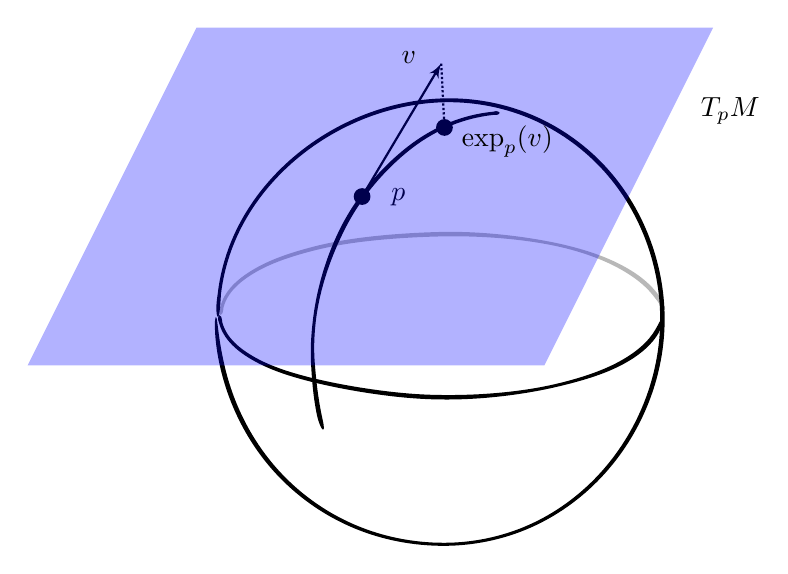
\begin{tikzpicture}[y=0.80pt, x=0.8pt,yscale=-1,scale=0.6, inner sep=0pt, outer sep=0pt]
\begin{scope}[shift={(-160.96945,-333.1402)}]% layer1
  % path53-7
  \path[fill=black] (303.8942,578.4579) .. controls (309.8492,613.6436) and
    (326.2950,647.0069) .. (351.2788,672.4277) .. controls (351.2788,672.4277) and
    (351.2788,672.4277) .. (351.2788,672.4277) .. controls (366.8467,688.2599) and
    (385.5450,700.9903) .. (405.9931,709.6300) .. controls (405.9931,709.6300) and
    (405.9931,709.6300) .. (405.9931,709.6300) .. controls (427.6728,718.7868) and
    (451.2361,723.2874) .. (474.7404,723.2020) .. controls (474.7404,723.2020) and
    (474.7404,723.2020) .. (474.7404,723.2020) .. controls (477.9402,723.1906) and
    (481.1397,723.0843) .. (484.3331,722.8835) .. controls (504.5069,721.6149) and
    (524.4437,716.6513) .. (542.7490,708.0802) .. controls (562.8258,698.6760) and
    (580.8698,685.0583) .. (595.6798,668.5587) .. controls (595.6798,668.5587) and
    (595.6798,668.5587) .. (595.6798,668.5587) .. controls (610.3628,652.2010) and
    (621.9135,633.0457) .. (629.6071,612.4429) .. controls (636.6571,593.5667) and
    (640.4575,573.4477) .. (640.5275,553.2944) .. controls (640.5345,551.4158) and
    (640.5091,549.5369) .. (640.4524,547.6587) .. controls (640.4524,547.6587) and
    (640.4524,547.6587) .. (640.4524,547.6587) .. controls (639.8181,526.7061) and
    (635.2651,505.8906) .. (627.1923,486.5436) .. controls (619.1195,467.1965) and
    (607.5233,449.3192) .. (592.7986,434.3077) .. controls (592.7986,434.3077) and
    (592.7986,434.3077) .. (592.7986,434.3077) .. controls (578.4290,419.6655) and
    (561.2422,407.7595) .. (542.3987,399.5509) .. controls (542.3987,399.5509) and
    (542.3987,399.5509) .. (542.3987,399.5509) .. controls (523.6843,391.4015) and
    (503.3886,386.9535) .. (482.9971,386.3768) .. controls (482.0345,386.3496) and
    (481.0717,386.3308) .. (480.1089,386.3205) .. controls (457.8237,386.0850) and
    (435.5966,390.4375) .. (414.8846,398.4803) .. controls (394.0725,406.5591) and
    (374.7216,418.3488) .. (358.0742,433.1676) .. controls (358.0742,433.1676) and
    (358.0742,433.1676) .. (358.0742,433.1676) .. controls (341.5295,447.8922) and
    (327.6569,465.6852) .. (318.0244,485.5977) .. controls (318.0244,485.5977) and
    (318.0244,485.5977) .. (318.0243,485.5977) .. controls (310.6484,500.8492) and
    (305.8685,517.3394) .. (304.0085,534.1311) .. controls (303.0434,539.8803) and
    (302.9573,544.1851) .. (303.1593,546.9729) .. controls (303.3614,549.7606) and
    (303.8508,551.0442) .. (304.3118,550.9077) .. controls (304.7728,550.7713) and
    (305.2084,549.2225) .. (305.5580,546.3461) .. controls (305.9076,543.4698) and
    (306.1732,539.2685) .. (306.5079,533.7492) .. controls (308.4195,517.4715) and
    (313.1243,501.4945) .. (320.3059,486.7165) .. controls (320.3059,486.7165) and
    (320.3059,486.7165) .. (320.3059,486.7165) .. controls (329.8132,467.1465) and
    (343.5170,449.6521) .. (359.8435,435.1730) .. controls (359.8435,435.1730) and
    (359.8435,435.1730) .. (359.8435,435.1730) .. controls (376.2770,420.6014) and
    (395.3751,409.0198) .. (415.8914,401.1018) .. controls (436.3086,393.2240) and
    (458.1883,388.9803) .. (480.0688,389.2588) .. controls (480.4777,389.2638) and
    (480.8867,389.2707) .. (481.2956,389.2790) .. controls (501.8630,389.6956) and
    (522.3603,394.1244) .. (541.1810,402.3707) .. controls (541.1810,402.3707) and
    (541.1810,402.3707) .. (541.1810,402.3707) .. controls (559.6426,410.4578) and
    (576.4777,422.1751) .. (590.5345,436.5541) .. controls (590.5345,436.5541) and
    (590.5346,436.5541) .. (590.5346,436.5541) .. controls (604.9389,451.2814) and
    (616.2760,468.8373) .. (624.1621,487.8256) .. controls (632.0482,506.8139) and
    (636.4871,527.2331) .. (637.0888,547.7557) .. controls (637.0888,547.7557) and
    (637.0888,547.7557) .. (637.0888,547.7557) .. controls (637.1046,548.2911) and
    (637.1177,548.8266) .. (637.1282,549.3622) .. controls (637.5334,570.0012) and
    (633.9588,591.2187) .. (626.5638,611.3090) .. controls (619.1596,631.4190) and
    (607.9362,650.4137) .. (593.5541,666.6562) .. controls (593.5541,666.6562) and
    (593.5541,666.6562) .. (593.5541,666.6562) .. controls (579.0427,683.0437) and
    (561.2751,696.5901) .. (541.7141,705.8690) .. controls (523.0585,714.7226) and
    (502.8189,719.6020) .. (482.8490,720.6839) .. controls (480.1405,720.8306) and
    (477.4365,720.9067) .. (474.7403,720.9131) .. controls (451.0493,720.9678) and
    (427.9571,716.2525) .. (407.0151,707.2248) .. controls (386.8523,698.5356) and
    (368.6767,685.8965) .. (353.5108,670.2453) .. controls (342.5872,658.9776) and
    (333.3083,646.1156) .. (325.8225,632.0701) .. controls (318.3366,618.0246) and
    (312.6396,602.7902) .. (309.0380,586.7495) .. controls (308.1977,583.0966) and
    (307.2183,578.4496) .. (306.3937,573.7010) .. controls (305.5691,568.9524) and
    (304.9020,564.1044) .. (304.4008,560.1034) .. controls (303.8996,556.1024) and
    (303.5458,552.9495) .. (303.1776,551.6125) .. controls (302.9935,550.9440) and
    (302.8047,550.7297) .. (302.6081,551.0931) .. controls (302.4116,551.4565) and
    (302.2056,552.3976) .. (302.0261,554.0418) .. controls (301.8778,557.6426) and
    (301.9897,561.7469) .. (302.3294,565.9485) .. controls (302.6691,570.1500) and
    (303.2369,574.4470) .. (303.8942,578.4579) -- cycle;

  % path57-2
  \path[fill=black] (382.9367,627.6720) .. controls (379.8377,613.7131) and
    (378.1962,599.3809) .. (377.0947,585.0162) .. controls (376.3205,574.9337) and
    (376.7152,564.7560) .. (377.8565,554.6494) .. controls (377.9525,553.7977) and
    (378.0557,552.9468) .. (378.1653,552.0967) .. controls (379.7024,540.1899) and
    (382.5553,528.4509) .. (386.3383,517.0366) .. controls (386.3383,517.0366) and
    (386.3383,517.0366) .. (386.3383,517.0366) .. controls (390.0178,505.9367) and
    (394.5805,495.1398) .. (399.8539,484.7028) .. controls (400.2371,483.9445) and
    (400.6261,483.1891) .. (401.0208,482.4369) .. controls (401.0208,482.4369) and
    (401.0208,482.4369) .. (401.0208,482.4369) .. controls (406.8903,471.2532) and
    (414.0278,460.7494) .. (422.1134,451.1037) .. controls (429.2175,442.6298) and
    (437.0493,434.8124) .. (445.4915,427.7518) .. controls (446.5098,426.9002) and
    (447.5397,426.0623) .. (448.5813,425.2388) .. controls (448.5813,425.2388) and
    (448.5813,425.2388) .. (448.5813,425.2388) .. controls (458.1231,417.6947) and
    (468.6510,411.3642) .. (479.9250,406.7785) .. controls (490.0069,402.6755) and
    (500.6879,399.9903) .. (511.5599,398.8282) .. controls (513.2711,398.9734) and
    (514.4966,398.8122) .. (515.2906,398.4921) .. controls (516.0845,398.1715) and
    (516.4441,397.6916) .. (516.3847,397.2327) .. controls (516.3257,396.7737) and
    (515.8437,396.3360) .. (514.9591,396.1270) .. controls (514.0746,395.9180) and
    (512.7843,395.9385) .. (511.1527,396.4170) .. controls (500.1103,397.5373) and
    (489.2447,400.1938) .. (478.9587,404.2940) .. controls (467.3925,408.9064) and
    (456.5869,415.2938) .. (446.7954,422.9321) .. controls (446.7954,422.9321) and
    (446.7954,422.9321) .. (446.7954,422.9321) .. controls (445.8533,423.6670) and
    (444.9204,424.4133) .. (443.9967,425.1706) .. controls (435.1883,432.3913) and
    (427.0243,440.4046) .. (419.6420,449.1100) .. controls (419.6420,449.1100) and
    (419.6420,449.1100) .. (419.6420,449.1100) .. controls (411.3562,458.8799) and
    (404.0450,469.5251) .. (398.0494,480.8641) .. controls (398.0494,480.8641) and
    (398.0494,480.8641) .. (398.0494,480.8641) .. controls (397.8298,481.2794) and
    (397.6120,481.6955) .. (397.3959,482.1127) .. controls (391.9193,492.6845) and
    (387.2296,504.2554) .. (383.5892,516.1412) .. controls (379.9767,527.9332) and
    (377.3931,540.0405) .. (375.9038,551.7786) .. controls (375.7771,552.7759) and
    (375.6580,553.7707) .. (375.5467,554.7626) .. controls (374.3793,565.1597) and
    (373.8040,575.2138) .. (374.3004,585.2101) .. controls (374.6322,591.9063) and
    (375.0692,598.5807) .. (375.7866,605.3085) .. controls (376.5037,612.0362) and
    (377.5008,618.8193) .. (378.9794,625.6952) .. controls (379.4880,627.8737) and
    (380.5229,631.1599) .. (381.5726,633.3646) .. controls (382.6224,635.5692) and
    (383.6492,636.6929) .. (384.0580,634.6606) .. controls (384.0268,632.5384) and
    (383.4029,629.9680) .. (382.9367,627.6720) -- cycle;

  % path59-5
  \path[fill=black] (633.4562,560.5798) .. controls (632.1456,562.8000) and
    (630.6312,564.9202) .. (628.9629,566.9166) .. controls (628.9629,566.9166) and
    (628.9629,566.9166) .. (628.9629,566.9166) .. controls (624.9501,571.7174) and
    (620.0493,575.8204) .. (614.7691,579.3837) .. controls (614.7691,579.3837) and
    (614.7691,579.3837) .. (614.7691,579.3837) .. controls (602.3861,587.7412) and
    (588.1118,593.1655) .. (573.5917,597.4195) .. controls (573.5917,597.4195) and
    (573.5917,597.4195) .. (573.5917,597.4195) .. controls (568.3949,598.9391) and
    (563.1492,600.2957) .. (557.8669,601.5182) .. controls (546.7227,604.0973) and
    (535.3783,605.8899) .. (523.9855,607.1746) .. controls (508.0451,608.9708) and
    (491.9969,609.7628) .. (475.9581,609.6914) .. controls (475.9581,609.6914) and
    (475.9581,609.6914) .. (475.9581,609.6914) .. controls (473.6715,609.6813) and
    (471.3848,609.6554) .. (469.0982,609.6151) .. controls (454.3721,609.3553) and
    (439.6704,608.0071) .. (425.0708,606.0621) .. controls (410.1302,604.0698) and
    (395.2952,601.4591) .. (380.6497,598.1524) .. controls (377.1339,597.3586) and
    (373.6321,596.5057) .. (370.1469,595.5880) .. controls (370.1469,595.5880) and
    (370.1469,595.5880) .. (370.1469,595.5880) .. controls (354.5537,591.4636) and
    (339.0784,586.3480) .. (325.8078,577.4741) .. controls (325.8078,577.4741) and
    (325.8078,577.4741) .. (325.8078,577.4741) .. controls (320.6148,573.9977) and
    (315.7933,569.9116) .. (312.2216,564.8660) .. controls (312.2216,564.8660) and
    (312.2216,564.8660) .. (312.2216,564.8660) .. controls (310.1612,561.9598) and
    (308.5611,558.7009) .. (307.5979,555.2683) .. controls (307.3721,553.2581) and
    (307.1116,551.8541) .. (306.7435,550.9272) .. controls (306.3754,550.0002) and
    (305.9027,549.5580) .. (305.4443,549.6278) .. controls (304.9859,549.6975) and
    (304.5435,550.2948) .. (304.4050,551.4154) .. controls (304.2664,552.5360) and
    (304.4416,554.1929) .. (305.3080,556.1270) .. controls (306.3309,559.7664) and
    (308.0013,563.2075) .. (310.1573,566.2797) .. controls (310.1573,566.2797) and
    (310.1573,566.2797) .. (310.1573,566.2797) .. controls (313.9550,571.6796) and
    (318.9732,576.0162) .. (324.3288,579.6243) .. controls (324.3288,579.6243) and
    (324.3288,579.6243) .. (324.3288,579.6243) .. controls (337.9560,588.8158) and
    (353.6867,594.1561) .. (369.3877,598.3706) .. controls (369.3877,598.3706) and
    (369.3877,598.3706) .. (369.3877,598.3706) .. controls (372.7165,599.2665) and
    (376.0595,600.1037) .. (379.4145,600.8869) .. controls (394.3606,604.3764) and
    (409.4865,607.1392) .. (424.6980,609.2404) .. controls (438.9101,611.2053) and
    (453.2345,612.5949) .. (467.6000,612.9520) .. controls (470.3548,613.0205) and
    (473.1345,613.0574) .. (475.9339,613.0611) .. controls (491.7629,613.0818) and
    (508.1947,611.9237) .. (524.2903,609.8127) .. controls (536.0926,608.2661) and
    (547.7395,606.2116) .. (558.8298,603.6372) .. controls (564.0744,602.4198) and
    (569.2057,601.1316) .. (574.2503,599.7334) .. controls (574.2503,599.7334) and
    (574.2503,599.7334) .. (574.2503,599.7334) .. controls (581.7164,597.6671) and
    (589.0394,595.3728) .. (596.1319,592.5473) .. controls (603.2243,589.7219) and
    (610.0924,586.3668) .. (616.5865,582.1468) .. controls (622.0460,578.5986) and
    (627.2287,574.3717) .. (631.5773,569.1978) .. controls (632.6451,567.9275) and
    (633.6571,566.5972) .. (634.6001,565.2103) .. controls (635.3620,564.0547) and
    (636.2294,562.5252) .. (636.9556,560.9093) .. controls (637.6818,559.2934) and
    (638.2629,557.5939) .. (638.5853,556.1583) .. controls (638.9076,554.7228) and
    (638.9793,553.5575) .. (638.7935,552.9962) .. controls (638.6077,552.4349) and
    (638.1847,552.4841) .. (637.4029,553.3674) .. controls (636.7752,554.4227) and
    (636.1589,555.6421) .. (635.5073,556.8902) .. controls (634.8556,558.1383) and
    (634.1683,559.4152) .. (633.4562,560.5798) -- cycle;

  % path61-2
  \path[fill=black,opacity=0.280] (637.0974,536.1628) .. controls
    (635.5496,533.8034) and (633.8117,531.5811) .. (631.9305,529.5094) .. controls
    (631.9305,529.5094) and (631.9305,529.5094) .. (631.9305,529.5094) .. controls
    (627.4226,524.5444) and (622.1713,520.3852) .. (616.6171,516.8221) .. controls
    (616.6171,516.8221) and (616.6171,516.8221) .. (616.6171,516.8221) .. controls
    (603.6218,508.4866) and (589.0665,503.0510) .. (574.3365,498.9791) .. controls
    (574.3365,498.9791) and (574.3365,498.9791) .. (574.3365,498.9791) .. controls
    (569.0614,497.5179) and (563.7414,496.2374) .. (558.3879,495.1244) .. controls
    (547.0935,492.7762) and (535.6874,490.9841) .. (524.2410,489.6297) .. controls
    (508.2248,487.7333) and (492.0837,486.6978) .. (475.9403,486.8574) .. controls
    (475.9403,486.8574) and (475.9403,486.8574) .. (475.9403,486.8574) .. controls
    (473.6402,486.8802) and (471.3404,486.9254) .. (469.0416,486.9932) .. controls
    (454.2362,487.4293) and (439.4419,488.3104) .. (424.7017,489.8069) .. controls
    (409.6172,491.3364) and (394.5375,493.5182) .. (379.7693,497.1078) .. controls
    (376.2240,497.9695) and (372.6933,498.8934) .. (369.1805,499.8853) .. controls
    (369.1805,499.8853) and (369.1805,499.8853) .. (369.1805,499.8853) .. controls
    (353.4963,504.2953) and (337.7663,509.9347) .. (324.3480,519.4189) .. controls
    (324.3480,519.4189) and (324.3480,519.4189) .. (324.3480,519.4189) .. controls
    (319.0747,523.1417) and (314.1765,527.5900) .. (310.5736,533.0206) .. controls
    (310.5736,533.0206) and (310.5736,533.0206) .. (310.5736,533.0206) .. controls
    (308.4846,536.1734) and (306.9190,539.6808) .. (306.0363,543.3405) .. controls
    (305.2251,545.3141) and (305.1188,546.9190) .. (305.3003,547.9506) .. controls
    (305.4817,548.9821) and (305.9436,549.4572) .. (306.4062,549.4295) .. controls
    (306.8688,549.4018) and (307.3341,548.8869) .. (307.6883,547.9428) .. controls
    (308.0426,546.9987) and (308.2851,545.6314) .. (308.4494,543.7331) .. controls
    (309.2884,540.4501) and (310.7354,537.2883) .. (312.6379,534.4343) .. controls
    (312.6379,534.4343) and (312.6379,534.4343) .. (312.6379,534.4343) .. controls
    (316.0148,529.3580) and (320.7163,525.1603) .. (325.8270,521.5691) .. controls
    (325.8270,521.5691) and (325.8270,521.5691) .. (325.8270,521.5691) .. controls
    (338.8888,512.4024) and (354.3639,506.9876) .. (369.9397,502.6679) .. controls
    (369.9397,502.6679) and (369.9397,502.6679) .. (369.9397,502.6679) .. controls
    (373.2381,501.7554) and (376.5531,500.9033) .. (379.8821,500.1065) .. controls
    (394.7126,496.5572) and (409.8811,494.4504) .. (425.0745,492.9852) .. controls
    (439.2699,491.6180) and (453.4970,490.8122) .. (467.7166,490.4013) .. controls
    (470.4434,490.3225) and (473.1942,490.2633) .. (475.9645,490.2271) .. controls
    (491.6140,490.0219) and (507.9032,490.6662) .. (523.9361,492.2677) .. controls
    (535.6930,493.4435) and (547.3124,495.1234) .. (558.3708,497.4519) .. controls
    (563.6003,498.5530) and (568.6951,499.8369) .. (573.6779,501.2929) .. controls
    (573.6779,501.2929) and (573.6779,501.2929) .. (573.6779,501.2929) .. controls
    (581.0559,503.4520) and (588.2199,505.9618) .. (595.0946,508.9569) .. controls
    (601.9692,511.9521) and (608.5554,515.4263) .. (614.7996,519.5851) .. controls
    (620.0372,523.0731) and (625.0080,527.0428) .. (629.3160,531.7905) .. controls
    (630.3709,532.9531) and (631.3854,534.1650) .. (632.3492,535.4260) .. controls
    (633.1602,536.4547) and (634.1833,537.7638) .. (635.1859,539.1315) .. controls
    (636.1885,540.4991) and (637.1677,541.9268) .. (637.9993,543.1147) .. controls
    (638.8309,544.3026) and (639.5231,545.2485) .. (640.0263,545.5816) .. controls
    (640.5295,545.9148) and (640.8654,545.6268) .. (640.8292,544.3503) .. controls
    (640.5600,543.0376) and (640.0382,541.6090) .. (639.3727,540.2052) .. controls
    (638.7072,538.8014) and (637.8990,537.4236) .. (637.0974,536.1628) -- cycle;

  % path1916
  \path[shift={(1704.3321,-988.83153)},fill=black,nonzero rule]
    (-1285.2569,1449.0822)arc(0.000:180.000:6.302)arc(-180.000:0.000:6.302) --
    cycle;

  % path4971
  \path[draw=black,line join=miter,line cap=butt,line width=0.800pt,-latex']
    (412.7728,460.2505) -- (472.3319,360.2060);

  % path4973
  \path[shift={(1766.3321,-1040.8315)},fill=black,nonzero rule]
    (-1285.2569,1449.0822)arc(0.000:180.000:6.302)arc(-180.000:0.000:6.302) --
    cycle;

  % path4975
  \path[draw=black,dash pattern=on 0.80pt off 0.80pt,line join=miter,line
    cap=butt,miter limit=4.00,line width=0.800pt] (472.3319,360.2060) --
    (474.7728,408.2506);

  % text4977
  \path[fill=black] (434.73734,467.13629) node[above right] (text4977) {$p$};

  \begin{scope}[shift={(1791.988,-1095.8603)}]% g1848
    % rect1914
    \path[cm={{1.0,0.0,-0.44705,0.89451,(0.0,0.0)}},fill=c0000ff,opacity=0.300,nonzero
      rule,rounded corners=0.0000cm] (-789.7889,1597.5265) rectangle
      (-400.8539,1881.7282);

    % text4981
    \path[fill=black] (-1124.1246,1501.9481) node[above right] (text4981) {$T_pM$};

  \end{scope}
  % text4985
  \path[fill=black] (442.5524,359.95026) node[above right] (text4985) {$v$};

  % text4989
  \path[fill=black] (487.88492,430.53278) node[above right] (text4989)
    {$\exp_p(v)$};

\end{scope}

\end{tikzpicture}


\end{center}

\end{frame}
%%%%%%next-slide%%%%%
Następny lemat powie nam, że geodezyjne na powierzchni $M$ przechodzące przez punkt $p$ są obrazami prostych przechodzących przez środek $T_pM$ przy odwzorowaniu wykładniczym.
\begin{frame}

\begin{lemat}
Niech $M\subset \R^3$ będzie powierzchnią gładką i niech $p\in M$ będzie punktem. Niech ponadto $v\in E_p$ będzie wektorem stycznym do $M$. Wtedy krzywa $\zeta\colon(-\varrho_v,\varrho_v)\to M$ zdefiniowana przez
\[\zeta(s)=\exp_p(sv)\] jest geodezyjną spełniającą $\zeta(0)=p$ oraz $\zeta'(0)=v$. Jej długość na odcinku od $p$ do $\exp_p(v)$ jest równa $\|v\|$.
\end{lemat}


\textcolor{ared}{\textbf{Dowód:}}\\\pause 
Niech $\gamma_v\colon (-\varrho_v,\varrho_v)\to M$ będzie geodezyjną spełniającą: $\gamma_v(0)=p$, oraz $\gamma_v'(0)=v$. Ustalmy $s\in (-\varrho_v,\varrho_v)$ i zdefiniujmy $\widetilde{\gamma}\colon(-\varrho_v/s,\varrho_v/s)\to M$ jako \[\widetilde{\gamma}(t)=\gamma_v(st).\]

\end{frame}
%%%%%%next-slide%%%%%
\begin{frame}
Ponieważ funkcja $t\to st$ jest liniowa, więc z charakteryzacji parametryzacji krzywych geodezyjnych (lemat \ref{lem:param-of-geodesics}) wynika, że $\widetilde{\gamma}$ jest również geodezyjną. Oczywiście $\widetilde{\gamma}(0)=p$ i $\widetilde{\gamma}'(0)=sv$.

\pause Mamy teraz:
\[\zeta(s)=\exp_p(sv)=\widetilde{\gamma}(1)=\gamma_v(s)\]
dla wszystkich $s\in (-\varrho_v, \varrho_v)$. Zatem $\zeta\equiv\gamma_v$ jest geodezyjną (korzystamy tutaj z jedyności!).

\pause Przypomnijmy, że geodezyjne mają stałą prędkość, więc
\[\|\zeta'(s)\|=\|\zeta'(0)\|=\|\gamma'(0)\|=\|v\|\]dla wszystkich $s$. Zatem długość geodezyjnej można policzyć jako
\[\int_0^1\|\zeta'(s)\|ds=\|v\|\int_0^1ds=\|v\|.\]
\hfill $\square$

\end{frame}
%%%%%%next-slide%%%%%

Widzieliśmy już na przykładzie sfery, że odwzorowanie wykładnicze nie jest injekcją. W każdym punkcie $p\in S^2$ sfery mamy $E_p=T_pS^2$, jednak proste na płaszczyźnie odwzorowywane na okręgi wielkie na sferze muszą się w pewnym momencie na siebie ``nawinąć''. Powinniśmy jednak zauważyć, że jeśli ograniczymy się do odpowiednio małego dysku w $T_pS^2$, jego obraz przy odwzorowaniu wykładniczym nie powinien wykraczać poza hemisferę zawierającą punkt $p$. Jest to fakt znacznie ogólniejszy.


\begin{frame}
Przypomnijmy, że przez $D(T_pM,\delta)$ oznaczamy dysk o środku w punkcie $\mathcal{O}=(0,0)\in T_pM$ i promieniu $\delta$.

%Następny lemat pokazuje, że jeśli jednak ograniczymy sie do odpowiednio niewielkiego otoczenia $\mathcal{O}\subset T_pM$dysku $D_{\mathcal{O}}(\delta_p,T_pM)$

\begin{lemat}
Niech $M\subset \R^3$ będzie powierzchnią gładką i niech $p\in M$. Istnieje wtedy taka $\delta>0$, że 
\begin{itemize} 
\item zbiór $\exp_p(D(T_pM,\delta)$ jest otwarty w $M$, oraz
\pause \item odwzorowanie wykładnicze \[\exp_p\big|_{D(T_pM,\delta_p)}\] ograniczone do zbioru $D(T_pM,\delta_p)$ jest dyfeomorfizmem na swój obraz.
\end{itemize}
\end{lemat}

\pause
% \begin{lemat}
% Istnieją również: otoczenie otwarte $W\subset M$ zawierające $p$, oraz liczba rzeczywista $\delta_p>0$ takie, że dla każdego $q\in W$ \[W\subset\exp_q(D(T_qM,\delta_p)).\]
% \end{lemat}

\end{frame}
%%%%%%next-slide%%%%%
\begin{frame}

\mode<article>{Jeśli $M$ jest powierzchnią zamkniętą (tj. zwartą i bez brzegu), wtedy korzystając ze zwartości można wykazać, że istnieje jedna uniwersalna stała $\delta_M$ zależna tylko od $M$, którą można podstawić w miejsce $\delta$ (zależną od punktu) w powyższych stwierdzeniach.}

\begin{uwaga}
Widzimy, że $\exp_p\colon D(T_pM,\delta_p)\to M$ jest dyfeomorfizmem na swój obraz. Nietrudno sprawdzić, że jest to przykład lokalnego układu współrzędnych na $M$ ($D(T_pM,\delta)\cong D^2\subset \R^2$). 
\end{uwaga}

\pause\begin{wniosek}
Niech $M\subset\R^3$ będzie powierzchnią gładką i niech $p\in M$ będzie punktem na niej. Ustalmy $0<\varepsilon<\delta$. Wtedy istnieje $V\subset M$ -- otwarte otoczenie punktu $p$, które posiada następujące własności:
\begin{itemize}
\item $V\subset \exp_q(D(T_qM,\varepsilon))$ dla wszstkich $q\in V$.
\pause \item każde dwa punkty w $V$ można połączyć krzywą geodezyjną o długości mniejszej niż $\varepsilon$.
\end{itemize}
\end{wniosek}

\end{frame}
%%%%%%next-slide%%%%%
\begin{frame}

\begin{uwaga}
Płaszczyzna ma tę własność, że wokół każdego punktu istnieje wypukłe otoczenie otwarte, tj. otoczenie w którym każde dwa punkty można połączyć odcinkiem geodezyjnej (czyli odcinkiem prostej). Tę własność nazywamy \textbf{wypukłością geodezyjną} i (co nie jest do końca oczywiste) posiada ją każda powierzchnia.
\end{uwaga}

\end{frame}
%%%%%%next-slide%%%%%
\mode<all>{\midsection{Triangulacje}}

\begin{frame}{Triangulacja}
\begin{definicja}
Niech $M\subset \R^3$ będzie powierzchnią gładką, i niech $x$, $y$, $z\in M$ będą różnymi punktami. Podzbiór $T\subset M$ nazywamy \textbf{trójkątem geodezyjnym} o wierzchołkach $x$, $y$, $z$ i oznaczamy $\vartriangle xyz$ jeśli $T$ jest homeomorficzny z dyskiem jednostkowym $D^2=\{(x,y)\in \R^2\colon x^2+y^2\leqslant1\}$, oraz brzeg $T$ oznaczany jako $\partial T$ składa się z trzech krzywych geodezyjnych $\overline{xy}$, $\overline{yz}$, $\overline{xz}$ (o końcach w $x$, $y$, $z$). \pause Te geodezyjne nazywamy \textbf{krawędziami} trójkąta geodezyjnego $\vartriangle xyz$. 
\end{definicja}

\end{frame}
%%%%%%next-slide%%%%%
% \begin{frame}
% @@@@ Rysunek @@@@
% \end{frame}
%%%%%%next-slide%%%%%
\begin{frame}

\begin{definicja}
Niech $\mathcal{T}$ będzie (skończoną) rodziną trójkątów geodezyjnch na $M$. Załóżmy, że dla wszystkie trójkąty w $\mathcal{T}$ są różne i każdy punkt $x\in M$ należy do pewnego trójkąta z $\mathcal{T}$. Rodzinę $\mathcal{T}$ nazywamy \textbf{triangulacją} powierzchni $M$ jeśli dla dowolnych dwóch trójkątów $T_1$, $T_2\in \mathcal{T}$ mamy 
\begin{itemize}
\item $T_1\cap T_2=\{x\}$ i $x$ jest ich wspólnym wierzchołkiem, lub
\pause\item $T_1\cap T_2=\{\overline{xy}\}$, gdzie $\overline{xy}$ jest ich wspólną krawędzią, lub
\pause\item $T_1\cap T_2=\varnothing$.
\end{itemize}
\end{definicja}

\pause \begin{lemat}
Dla każdego $\varepsilon>0$ istnieje triangulacja geodezyjna $\mathcal{T}$ zwartej powierzchni $M\subset \R^3$ w której każdy trójkąt geodezyjny ma średnicę mniejszą od $\varepsilon$.
\end{lemat}
\end{frame}
%%%%%%next-slide%%%%%
\begin{frame}

\begin{przyklad}
Triangulacja geodezyjna sfery $S^2$.
\begin{center}

\definecolor{c800080}{RGB}{128,0,128}
\definecolor{c999999}{RGB}{153,153,153}
\definecolor{c0000ff}{RGB}{0,0,255}
\definecolor{c00ff00}{RGB}{0,255,0}
\definecolor{cff0000}{RGB}{255,0,0}


\begin{tikzpicture}[y=0.80pt, x=0.8pt,yscale=-1,scale=0.7, inner sep=0pt, outer sep=0pt]
\begin{scope}[shift={(127.98735,-96.41156)}]% layer1
  \begin{scope}[shift={(-104.19343,-503.86607)}]% g5663
    % path5616
    \path[fill=c800080,opacity=0.300,nonzero rule] (164.3624,704.2777) .. controls
      (153.7670,711.9457) and (143.5951,719.9259) .. (133.9249,727.9964) .. controls
      (118.9774,740.4737) and (105.2645,753.1550) .. (92.8937,765.6214) --
      (90.3624,768.1839) .. controls (89.0169,769.5570) and (87.6745,770.9428) ..
      (86.3624,772.3089) .. controls (84.7775,773.9594) and (83.2110,775.6071) ..
      (81.6749,777.2464) .. controls (70.8899,788.7584) and (61.0474,800.2740) ..
      (52.4874,811.5589) -- (50.5812,814.0902) .. controls (49.9529,814.9353) and
      (49.3194,815.7789) .. (48.7062,816.6214) .. controls (39.5341,829.2264) and
      (31.9908,841.5607) .. (27.4562,852.8714) .. controls (23.7250,862.1977) and
      (21.9570,870.9383) .. (24.3937,877.3402) .. controls (24.4586,877.5053) and
      (24.5162,877.6484) .. (24.5812,877.8089) .. controls (26.0028,878.9557) and
      (27.7570,881.0344) .. (29.7062,884.4027) -- (30.7687,887.2464) .. controls
      (45.3084,901.5060) and (62.4208,913.0614) .. (81.2687,921.1839) .. controls
      (102.2107,930.2116) and (125.2963,934.9260) .. (148.9874,934.8714) .. controls
      (151.6836,934.8654) and (154.3726,934.7994) .. (157.0812,934.6527) .. controls
      (172.8177,933.8001) and (188.7292,930.5892) .. (203.8937,924.9339) .. controls
      (205.6951,923.0952) and (207.2564,920.7923) .. (209.3624,919.4027) .. controls
      (212.8112,917.1270) and (215.5233,914.0228) .. (217.6437,910.4964) .. controls
      (223.3202,901.0500) and (225.3204,889.2893) .. (226.1749,877.3089) .. controls
      (227.2910,861.3936) and (225.9539,844.7334) .. (223.4249,827.9339) .. controls
      (223.0240,825.2740) and (222.5765,822.6021) .. (222.1124,819.9339) --
      (221.7062,817.6527) .. controls (219.2879,804.2452) and (216.0928,790.7546) ..
      (212.2999,777.2464) -- (211.7687,775.3089) .. controls (211.6112,774.7565) and
      (211.4594,774.2052) .. (211.2999,773.6527) .. controls (210.7137,771.6202) and
      (210.1061,769.5738) .. (209.4874,767.5277) .. controls (203.5097,747.7638) and
      (196.0266,727.4081) .. (186.7062,707.1527) .. controls (186.4043,706.4969) and
      (186.1055,705.8395) .. (185.7999,705.1839) .. controls (178.6278,704.6863) and
      (171.4659,704.4162) .. (164.3624,704.2777) -- cycle;

    % path1985-9-0
    \path[fill=c999999,nonzero rule] (103.7062,610.4339) .. controls
      (99.2433,610.4228) and (100.3365,612.6375) .. (104.3937,612.6526) .. controls
      (107.5784,612.6534) and (110.9914,613.3785) .. (114.3624,614.6526) .. controls
      (115.2273,614.9795) and (116.0707,615.3525) .. (116.9249,615.7464) .. controls
      (121.7126,617.9529) and (126.2983,621.1022) .. (130.5812,624.6526) .. controls
      (141.8230,633.9747) and (151.0517,645.7187) .. (159.2999,657.8089) .. controls
      (166.8959,668.9643) and (173.5337,680.5843) .. (179.5187,692.3401) .. controls
      (175.1862,695.1948) and (170.9111,698.0922) .. (166.7062,701.0589) .. controls
      (161.2016,700.8482) and (155.6849,700.7544) .. (150.1749,700.8089) .. controls
      (147.8747,700.8317) and (145.5988,700.8974) .. (143.2999,700.9651) .. controls
      (128.4945,701.4013) and (113.6964,702.2812) .. (98.9562,703.7776) .. controls
      (83.8717,705.3071) and (68.7868,707.4693) .. (54.0187,711.0589) .. controls
      (50.4733,711.9206) and (46.9378,712.8483) .. (43.4249,713.8401) .. controls
      (27.7407,718.2501) and (11.9994,723.8872) .. (-1.4188,733.3714) .. controls
      (-6.6921,737.0942) and (-11.5659,741.5658) .. (-15.1688,746.9964) .. controls
      (-17.2578,750.1492) and (-18.8487,753.6492) .. (-19.7313,757.3089) .. controls
      (-20.5425,759.2826) and (-20.6315,760.8711) .. (-20.4501,761.9026) .. controls
      (-20.2686,762.9342) and (-19.8190,763.4303) .. (-19.3563,763.4026) .. controls
      (-18.8937,763.3749) and (-18.4293,762.8468) .. (-18.0751,761.9026) .. controls
      (-17.7209,760.9585) and (-17.4581,759.5822) .. (-17.2938,757.6839) .. controls
      (-16.4548,754.4008) and (-15.0089,751.2566) .. (-13.1063,748.4026) .. controls
      (-9.7295,743.3263) and (-5.0296,739.1188) .. (0.0812,735.5276) .. controls
      (13.1430,726.3609) and (28.5991,720.9411) .. (44.1749,716.6214) .. controls
      (47.4733,715.7089) and (50.7834,714.8556) .. (54.1124,714.0589) .. controls
      (68.9429,710.5095) and (84.1377,708.4303) .. (99.3312,706.9651) .. controls
      (113.5265,705.5980) and (127.7366,704.7822) .. (141.9562,704.3714) .. controls
      (144.6830,704.2926) and (147.4358,704.2201) .. (150.2062,704.1839) .. controls
      (154.1898,704.1317) and (158.2169,704.1555) .. (162.2687,704.2152) .. controls
      (151.8309,711.7468) and (141.8003,719.5675) .. (132.2374,727.4964) .. controls
      (114.5567,742.1543) and (98.3824,757.2433) .. (83.9249,772.3089) .. controls
      (83.0224,773.2471) and (82.1249,774.1833) .. (81.2374,775.1214) .. controls
      (67.8779,789.2477) and (55.8951,803.3742) .. (45.8937,817.1527) .. controls
      (36.6252,829.9186) and (29.0115,842.4450) .. (24.4249,853.9652) .. controls
      (20.6311,863.4706) and (18.8847,872.4227) .. (21.4249,879.0589) .. controls
      (32.2885,888.7781) and (28.2282,887.0914) .. (24.3937,877.3402) .. controls
      (21.9570,870.9383) and (23.7250,862.1977) .. (27.4562,852.8714) .. controls
      (31.9908,841.5607) and (39.5341,829.2264) .. (48.7062,816.6214) .. controls
      (58.0997,803.7165) and (69.2665,790.4912) .. (81.6749,777.2464) .. controls
      (83.2110,775.6071) and (84.7775,773.9594) .. (86.3624,772.3089) .. controls
      (100.3709,757.7226) and (116.2999,742.7086) .. (133.9249,727.9964) .. controls
      (143.5951,719.9260) and (153.7670,711.9457) .. (164.3624,704.2777) .. controls
      (171.4659,704.4162) and (178.6278,704.6863) .. (185.7999,705.1839) .. controls
      (186.1055,705.8395) and (186.4043,706.4969) .. (186.7062,707.1527) .. controls
      (196.0266,727.4081) and (203.5097,747.7638) .. (209.4874,767.5277) .. controls
      (210.1061,769.5738) and (210.7137,771.6202) .. (211.2999,773.6527) .. controls
      (216.5419,791.8166) and (220.7183,809.9768) .. (223.4249,827.9339) .. controls
      (225.9539,844.7334) and (227.2910,861.3936) .. (226.1749,877.3089) .. controls
      (225.3204,889.2893) and (223.3202,901.0500) .. (217.6437,910.4964) .. controls
      (215.5233,914.0228) and (212.8541,917.1935) .. (209.3624,919.4027) .. controls
      (207.0150,920.8889) and (202.2713,925.1585) .. (203.5812,924.9339) .. controls
      (206.5281,924.4288) and (209.2223,923.3578) .. (211.5187,921.9027) .. controls
      (215.3337,919.4823) and (218.2030,916.1343) .. (220.4249,912.4339) .. controls
      (226.3518,902.5746) and (228.4947,890.5125) .. (229.3624,878.3714) .. controls
      (230.5418,862.2212) and (229.2545,845.3761) .. (226.7374,828.4339) .. controls
      (223.9168,809.4317) and (219.4587,790.2295) .. (213.8312,771.0277) .. controls
      (213.4913,769.8691) and (213.1525,768.6863) .. (212.7999,767.5277) .. controls
      (206.6568,747.1655) and (198.9573,726.7916) .. (189.5187,706.6839) .. controls
      (189.3234,706.2678) and (189.1217,705.8499) .. (188.9249,705.4339) .. controls
      (192.0111,705.6714) and (195.1013,705.9394) .. (198.1749,706.2464) .. controls
      (209.9318,707.4221) and (221.5540,709.0742) .. (232.6124,711.4027) .. controls
      (237.8419,712.5038) and (242.9422,713.7904) .. (247.9249,715.2464) .. controls
      (255.3029,717.4055) and (262.4565,719.9388) .. (269.3312,722.9339) .. controls
      (276.2058,725.9291) and (282.8057,729.4001) .. (289.0499,733.5589) .. controls
      (294.2875,737.0469) and (299.2418,740.9987) .. (303.5499,745.7464) .. controls
      (304.6048,746.9090) and (305.6173,748.1417) .. (306.5812,749.4027) .. controls
      (307.3922,750.4314) and (308.4223,751.7225) .. (309.4249,753.0902) .. controls
      (310.4275,754.4579) and (311.4058,755.9023) .. (312.2374,757.0902) .. controls
      (313.0690,758.2781) and (313.7655,759.2258) .. (314.2687,759.5589) .. controls
      (314.7719,759.8921) and (315.1174,759.5855) .. (315.0812,758.3089) .. controls
      (314.8119,756.9963) and (314.2779,755.5877) .. (313.6124,754.1839) .. controls
      (312.9469,752.7802) and (312.1328,751.3822) .. (311.3312,750.1214) .. controls
      (309.7833,747.7620) and (308.0561,745.5369) .. (306.1749,743.4652) .. controls
      (301.6670,738.5003) and (296.4166,734.3408) .. (290.8624,730.7777) .. controls
      (277.8672,722.4423) and (263.3112,717.0058) .. (248.5812,712.9339) .. controls
      (243.3061,711.4728) and (237.9972,710.2032) .. (232.6437,709.0902) .. controls
      (221.3493,706.7420) and (209.9338,704.9446) .. (198.4874,703.5902) .. controls
      (194.8254,703.1566) and (191.1610,702.7735) .. (187.4874,702.4339) .. controls
      (185.7941,698.9230) and (184.0469,695.4238) .. (182.2374,691.9339) .. controls
      (182.3123,691.8848) and (182.3812,691.8268) .. (182.4562,691.7777) .. controls
      (196.7965,682.3855) and (211.8360,673.6954) .. (226.3937,667.3714) .. controls
      (232.7872,664.5925) and (239.0625,662.3052) .. (244.8624,660.7464) .. controls
      (247.0967,660.1456) and (249.2600,659.6513) .. (251.3312,659.2777) .. controls
      (254.4906,658.7078) and (257.4330,658.4068) .. (260.0812,658.4027) .. controls
      (264.5407,658.3937) and (268.1643,659.2319) .. (270.8624,660.7152) .. controls
      (273.7236,662.2863) and (275.9795,660.7264) .. (272.9874,659.1214) .. controls
      (270.1214,657.5864) and (266.2808,656.7595) .. (261.6437,656.7777) .. controls
      (258.5924,656.7911) and (255.2016,657.1698) .. (251.5812,657.8714) .. controls
      (249.6978,658.2364) and (247.7612,658.6803) .. (245.7687,659.2152) .. controls
      (239.6864,660.8490) and (233.2134,663.2288) .. (226.6749,666.0589) .. controls
      (211.5199,672.6221) and (196.1852,681.4441) .. (181.7062,690.8714) .. controls
      (181.7042,690.8674) and (181.6772,690.8754) .. (181.6749,690.8714) .. controls
      (175.6533,679.3473) and (168.9763,667.9607) .. (161.3624,656.9339) .. controls
      (153.0398,644.8641) and (143.5824,632.9394) .. (131.7999,623.1839) .. controls
      (127.3847,619.5273) and (122.5607,616.2035) .. (117.3936,613.8089) .. controls
      (116.8045,613.5361) and (116.2406,613.2718) .. (115.6436,613.0277) .. controls
      (111.6988,611.4148) and (107.5866,610.4588) .. (103.7062,610.4339) --
      cycle(180.0499,693.3714) .. controls (181.5245,696.2896) and
      (182.9685,699.2211) .. (184.3624,702.1526) .. controls (179.1658,701.7123) and
      (173.9485,701.3813) .. (168.7374,701.1526) .. controls (172.4632,698.5171) and
      (176.2294,695.9103) .. (180.0499,693.3714) -- cycle;

    % path5502-3
    \path[fill=c0000ff,opacity=0.300,nonzero rule] (259.8208,658.5285) .. controls
      (257.1726,658.5325) and (254.2302,658.8336) .. (251.0708,659.4035) .. controls
      (248.9996,659.7771) and (246.8363,660.2713) .. (244.6020,660.8722) .. controls
      (238.8021,662.4310) and (232.5268,664.7183) .. (226.1333,667.4972) .. controls
      (211.5756,673.8212) and (196.5361,682.5113) .. (182.1958,691.9035) .. controls
      (182.1209,691.9526) and (182.0519,692.0106) .. (181.9770,692.0597) .. controls
      (183.7865,695.5496) and (185.5337,699.0488) .. (187.2270,702.5597) .. controls
      (190.9006,702.8993) and (194.5650,703.2824) .. (198.2270,703.7160) .. controls
      (209.6734,705.0704) and (221.0889,706.8678) .. (232.3833,709.2160) .. controls
      (237.7368,710.3290) and (243.0457,711.5986) .. (248.3208,713.0597) .. controls
      (252.1833,714.1275) and (256.0384,715.3079) .. (259.8520,716.5910) --
      (261.8520,717.2785) .. controls (271.8784,720.7784) and (281.6106,725.1362) ..
      (290.6020,730.9035) .. controls (296.1562,734.4666) and (301.4066,738.6260) ..
      (305.9145,743.5910) .. controls (307.4410,745.2721) and (308.8543,747.0618) ..
      (310.1645,748.9347) .. controls (308.4293,732.8036) and (304.3628,716.9031) ..
      (298.1333,701.9035) .. controls (293.2443,690.1319) and (287.0521,678.9289) ..
      (279.6020,668.5910) .. controls (273.6737,662.6430) and (272.8746,657.9356) ..
      (259.8208,658.5285) -- cycle;

    % path5488-6
    \path[fill=c0000ff,opacity=0.500,nonzero rule] (279.6817,668.5757) .. controls
      (281.0729,674.8898) and (279.3159,682.8313) .. (275.9630,691.2320) .. controls
      (272.6761,699.4875) and (267.8226,708.2564) .. (261.9317,717.2632) --
      (260.4005,719.5445) .. controls (258.5163,722.3542) and (256.5575,725.2025) ..
      (254.4942,728.0445) .. controls (244.4928,741.8229) and (232.5099,755.9495) ..
      (219.1505,770.0757) .. controls (218.2630,771.0139) and (217.3655,771.9501) ..
      (216.4630,772.8882) .. controls (215.8757,773.5002) and (215.2746,774.1200) ..
      (214.6817,774.7320) -- (212.1192,777.3570) .. controls (198.7856,790.9352) and
      (184.0854,804.4902) .. (168.1505,817.7007) .. controls (165.7248,819.7119) and
      (163.2595,821.7062) .. (160.7755,823.7007) .. controls (173.2303,823.4556) and
      (185.6780,822.6581) .. (198.0567,821.2632) .. controls (205.9268,820.3758) and
      (213.7535,819.2272) .. (221.5255,817.7632) -- (224.6817,817.1695) .. controls
      (227.1034,816.6833) and (229.5267,816.1636) .. (231.9317,815.6070) .. controls
      (237.2140,814.3845) and (242.4537,813.0016) .. (247.6505,811.4820) .. controls
      (262.1705,807.2280) and (276.4549,801.8082) .. (288.8380,793.4507) .. controls
      (294.1182,789.8874) and (299.0127,785.7828) .. (303.0255,780.9820) .. controls
      (304.6938,778.9855) and (306.2148,776.8897) .. (307.5255,774.6695) .. controls
      (308.2376,773.5049) and (308.9050,772.2302) .. (309.5567,770.9820) .. controls
      (310.1187,769.9056) and (310.6714,768.8681) .. (311.2130,767.9195) .. controls
      (311.2250,766.4266) and (311.2110,764.9383) .. (311.1817,763.4507) .. controls
      (311.1711,762.9152) and (311.1663,762.3611) .. (311.1504,761.8257) .. controls
      (311.0877,759.6882) and (310.9834,757.5533) .. (310.8379,755.4195) --
      (310.2441,748.9195) .. controls (308.5091,732.7884) and (304.4425,716.8879) ..
      (298.2130,701.8882) .. controls (293.3240,690.1166) and (287.1318,678.9137) ..
      (279.6817,668.5757) -- cycle;

    % path5506-0
    \path[fill=c00ff00,opacity=0.300,nonzero rule] (102.0265,612.3445) --
      (89.5578,615.3132) .. controls (69.2685,623.2247) and (50.3627,634.7272) ..
      (34.0890,649.1570) .. controls (17.7625,663.6362) and (4.0650,681.1182) ..
      (-5.4422,700.6882) .. controls (-12.6238,715.4662) and (-17.3431,731.4418) ..
      (-19.2547,747.7195) .. controls (-19.5058,751.8589) and (-19.7044,755.2532) ..
      (-19.9422,757.9070) .. controls (-19.8716,757.7054) and (-19.8100,757.5238) ..
      (-19.7235,757.3132) .. controls (-18.8408,753.6536) and (-17.2500,750.1536) ..
      (-15.1610,747.0007) .. controls (-11.5581,741.5701) and (-6.6843,737.0985) ..
      (-1.4110,733.3757) .. controls (12.0073,723.8915) and (27.7486,718.2545) ..
      (43.4328,713.8445) .. controls (46.9456,712.8526) and (50.4812,711.9250) ..
      (54.0265,711.0632) .. controls (61.4006,709.2709) and (68.8465,707.8365) ..
      (76.3390,706.6570) -- (79.4953,706.1882) .. controls (85.9648,705.2317) and
      (92.4693,704.4405) .. (98.9640,703.7820) .. controls (113.7042,702.2856) and
      (128.5024,701.4056) .. (143.3078,700.9695) .. controls (145.6067,700.9018) and
      (147.8826,700.8360) .. (150.1828,700.8132) .. controls (155.6927,700.7587) and
      (161.2095,700.8525) .. (166.7140,701.0632) .. controls (170.9189,698.0965) and
      (175.1941,695.1992) .. (179.5265,692.3445) .. controls (173.5415,680.5887) and
      (166.9037,668.9686) .. (159.3078,657.8132) .. controls (151.0596,645.7231) and
      (141.8308,633.9790) .. (130.5890,624.6570) .. controls (126.3061,621.1066) and
      (121.7204,617.9572) .. (116.9328,615.7507) .. controls (116.0786,615.3568) and
      (115.2351,614.9839) .. (114.3703,614.6570) .. controls (110.9992,613.3829) and
      (107.5862,612.6577) .. (104.4015,612.6570) .. controls (103.4208,612.6533) and
      (102.6242,612.5427) .. (102.0265,612.3445) -- cycle;

    % path5490-8
    \path[fill=c00ff00,opacity=0.500,nonzero rule] (89.4725,615.1723) .. controls
      (69.1833,623.0838) and (50.2774,634.5863) .. (34.0038,649.0161) .. controls
      (17.6772,663.4952) and (3.9797,680.9773) .. (-5.5275,700.5473) .. controls
      (-12.7091,715.3253) and (-17.4284,731.3009) .. (-19.3400,747.5786) .. controls
      (-19.5911,751.7180) and (-19.7896,755.1123) .. (-20.0275,757.7661) .. controls
      (-20.0275,757.7661) and (-20.0548,760.3993) .. (-21.0275,763.9536) .. controls
      (-20.8443,763.6571) and (-20.6317,763.4885) .. (-20.4025,763.4536) .. controls
      (-19.9441,763.3839) and (-19.4581,763.8391) .. (-19.0900,764.7661) .. controls
      (-18.7219,765.6930) and (-18.4720,767.0996) .. (-18.2462,769.1098) .. controls
      (-17.2830,772.5423) and (-15.6817,775.7974) .. (-13.6212,778.7036) .. controls
      (-10.0495,783.7492) and (-5.2204,787.8209) .. (-0.0275,791.2973) .. controls
      (13.2431,800.1712) and (28.7230,805.2979) .. (44.3163,809.4223) .. controls
      (46.3183,809.9494) and (48.3358,810.4374) .. (50.3475,810.9223) --
      (52.4100,811.4223) .. controls (53.2132,811.6102) and (54.0113,811.8031) ..
      (54.8163,811.9848) .. controls (69.4617,815.2916) and (84.2819,817.8988) ..
      (99.2225,819.8911) .. controls (102.8198,820.3703) and (106.4265,820.8041) ..
      (110.0350,821.2036) .. controls (102.1852,803.6033) and (95.6457,785.8119) ..
      (90.2850,768.0473) -- (89.7225,766.1411) .. controls (89.5655,765.6108) and
      (89.4098,765.0792) .. (89.2538,764.5473) .. controls (83.8637,746.1558) and
      (79.5557,727.7635) .. (76.7225,709.5473) -- (76.2538,706.5161) .. controls
      (73.7979,689.7853) and (72.5576,673.1546) .. (73.7225,657.2036) .. controls
      (74.5903,645.0625) and (76.7331,633.0004) .. (82.6600,623.1411) .. controls
      (84.4509,620.1586) and (86.6843,617.4037) .. (89.4725,615.1723) -- cycle;

    % path5476-8
    \path[fill=cff0000,opacity=0.500,nonzero rule] (114.8937,825.1526) .. controls
      (123.8531,826.0761) and (132.8218,826.6787) .. (141.8312,826.9026) .. controls
      (144.5860,826.9711) and (147.3755,827.0239) .. (150.1749,827.0276) .. controls
      (151.6044,827.0296) and (153.0485,827.0136) .. (154.4874,826.9963) .. controls
      (145.3652,834.2093) and (135.8474,841.2591) .. (126.0187,847.9963) .. controls
      (122.6234,841.5607) and (119.4202,835.0657) .. (116.4249,828.5588) .. controls
      (115.9039,827.4266) and (115.4032,826.2855) .. (114.8937,825.1526) -- cycle;

    % path1979-2-8
    \path[fill=black] (-21.8615,792.4241) .. controls (-15.9065,827.6098) and
      (0.5392,860.9731) .. (25.5230,886.3939) .. controls (25.5230,886.3939) and
      (25.5230,886.3939) .. (25.5230,886.3939) .. controls (41.0910,902.2261) and
      (59.7893,914.9565) .. (80.2373,923.5962) .. controls (80.2373,923.5962) and
      (80.2373,923.5962) .. (80.2373,923.5962) .. controls (101.9170,932.7530) and
      (125.4803,937.2536) .. (148.9846,937.1682) .. controls (148.9846,937.1682) and
      (148.9846,937.1682) .. (148.9846,937.1682) .. controls (152.1844,937.1568) and
      (155.3839,937.0505) .. (158.5773,936.8497) .. controls (178.7511,935.5811) and
      (198.6879,930.6175) .. (216.9932,922.0464) .. controls (237.0700,912.6422) and
      (255.1140,899.0245) .. (269.9239,882.5249) .. controls (269.9239,882.5249) and
      (269.9239,882.5249) .. (269.9239,882.5249) .. controls (284.6070,866.1672) and
      (296.1577,847.0119) .. (303.8513,826.4092) .. controls (310.9013,807.5330) and
      (314.7018,787.4139) .. (314.7718,767.2607) .. controls (314.7788,765.3821) and
      (314.7534,763.5032) .. (314.6967,761.6249) .. controls (314.6967,761.6249) and
      (314.6967,761.6249) .. (314.6967,761.6249) .. controls (314.0623,740.6723) and
      (309.5094,719.8568) .. (301.4366,700.5098) .. controls (293.3638,681.1627) and
      (281.7676,663.2854) .. (267.0428,648.2739) .. controls (267.0428,648.2739) and
      (267.0428,648.2739) .. (267.0428,648.2739) .. controls (252.6732,633.6317) and
      (235.4865,621.7257) .. (216.6429,613.5171) .. controls (216.6429,613.5171) and
      (216.6429,613.5171) .. (216.6429,613.5171) .. controls (197.9285,605.3677) and
      (177.6328,600.9197) .. (157.2413,600.3430) .. controls (156.2787,600.3158) and
      (155.3159,600.2970) .. (154.3531,600.2867) .. controls (132.0679,600.0512) and
      (109.8408,604.4037) .. (89.1288,612.4465) .. controls (68.3166,620.5253) and
      (48.9658,632.3150) .. (32.3184,647.1338) .. controls (32.3184,647.1338) and
      (32.3184,647.1338) .. (32.3184,647.1338) .. controls (15.7736,661.8584) and
      (1.9011,679.6514) .. (-7.7315,699.5639) .. controls (-7.7315,699.5639) and
      (-7.7315,699.5639) .. (-7.7315,699.5639) .. controls (-15.1075,714.8154) and
      (-19.8873,731.3056) .. (-21.7473,748.0973) .. controls (-22.7124,753.8465) and
      (-22.7985,758.1513) .. (-22.5965,760.9391) .. controls (-22.3944,763.7268) and
      (-21.9051,765.0105) .. (-21.4440,764.8740) .. controls (-20.9830,764.7375) and
      (-20.5474,763.1887) .. (-20.1978,760.3124) .. controls (-19.8482,757.4360) and
      (-19.5826,753.2347) .. (-19.2479,747.7154) .. controls (-17.3363,731.4377) and
      (-12.6315,715.4607) .. (-5.4499,700.6827) .. controls (-5.4499,700.6827) and
      (-5.4499,700.6827) .. (-5.4499,700.6827) .. controls (4.0573,681.1127) and
      (17.7611,663.6183) .. (34.0877,649.1392) .. controls (34.0877,649.1392) and
      (34.0877,649.1392) .. (34.0877,649.1392) .. controls (50.5212,634.5676) and
      (69.6193,622.9860) .. (90.1356,615.0680) .. controls (110.5528,607.1902) and
      (132.4325,602.9465) .. (154.3130,603.2250) .. controls (154.7220,603.2300) and
      (155.1309,603.2369) .. (155.5398,603.2452) .. controls (176.1072,603.6617) and
      (196.6046,608.0905) .. (215.4253,616.3368) .. controls (215.4253,616.3368) and
      (215.4253,616.3368) .. (215.4253,616.3368) .. controls (233.8869,624.4239) and
      (250.7220,636.1412) .. (264.7789,650.5203) .. controls (264.7789,650.5203) and
      (264.7789,650.5203) .. (264.7789,650.5203) .. controls (279.1832,665.2475) and
      (290.5203,682.8035) .. (298.4064,701.7918) .. controls (306.2925,720.7801) and
      (310.7314,741.1994) .. (311.3331,761.7220) .. controls (311.3331,761.7220) and
      (311.3331,761.7220) .. (311.3331,761.7220) .. controls (311.3489,762.2574) and
      (311.3620,762.7929) .. (311.3725,763.3284) .. controls (311.7776,783.9674) and
      (308.2030,805.1849) .. (300.8080,825.2752) .. controls (293.4037,845.3852) and
      (282.1804,864.3799) .. (267.7983,880.6224) .. controls (267.7983,880.6224) and
      (267.7983,880.6224) .. (267.7983,880.6224) .. controls (253.2869,897.0099) and
      (235.5194,910.5563) .. (215.9583,919.8353) .. controls (197.3027,928.6889) and
      (177.0631,933.5683) .. (157.0933,934.6502) .. controls (154.3847,934.7970) and
      (151.6807,934.8730) .. (148.9845,934.8794) .. controls (125.2935,934.9340) and
      (102.2013,930.2188) .. (81.2592,921.1911) .. controls (61.0964,912.5019) and
      (42.9209,899.8627) .. (27.7550,884.2115) .. controls (16.8314,872.9438) and
      (7.5525,860.0818) .. (0.0667,846.0363) .. controls (-7.4192,831.9908) and
      (-13.1162,816.7564) .. (-16.7178,800.7158) .. controls (-17.5581,797.0629) and
      (-18.5375,792.4158) .. (-19.3621,787.6672) .. controls (-20.1867,782.9186) and
      (-20.8538,778.0706) .. (-21.3550,774.0696) .. controls (-21.8562,770.0686) and
      (-22.2100,766.9157) .. (-22.5782,765.5787) .. controls (-22.7623,764.9102) and
      (-22.9512,764.6959) .. (-23.1477,765.0593) .. controls (-23.3443,765.4227) and
      (-23.5502,766.3638) .. (-23.7298,768.0080) .. controls (-23.8780,771.6088) and
      (-23.7661,775.7131) .. (-23.4264,779.9147) .. controls (-23.0866,784.1162) and
      (-22.5188,788.4132) .. (-21.8615,792.4241) -- cycle;

    % path1981-9-4
    \path[fill=black] (99.5499,610.7776) .. controls (96.6030,611.2828) and
      (93.9400,612.3226) .. (91.6437,613.7776) .. controls (87.8287,616.1980) and
      (84.9594,619.5773) .. (82.7374,623.2776) .. controls (76.8106,633.1370) and
      (74.6677,645.1991) .. (73.7999,657.3401) .. controls (72.6205,673.4904) and
      (73.9078,690.3354) .. (76.4249,707.2776) .. controls (79.2455,726.2799) and
      (83.7036,745.4820) .. (89.3312,764.6839) .. controls (89.6710,765.8425) and
      (90.0099,766.9941) .. (90.3624,768.1526) .. controls (95.7247,785.9267) and
      (102.2584,803.7304) .. (110.1124,821.3401) .. controls (106.5039,820.9407) and
      (102.8972,820.5069) .. (99.2999,820.0276) .. controls (84.3594,818.0353) and
      (69.5391,815.4281) .. (54.8937,812.1214) .. controls (51.3778,811.3275) and
      (47.8789,810.4765) .. (44.3937,809.5589) .. controls (28.8004,805.4344) and
      (13.3205,800.3078) .. (0.0499,791.4339) .. controls (-5.1430,787.9574) and
      (-9.9721,783.8858) .. (-13.5438,778.8401) .. controls (-15.6043,775.9340) and
      (-17.2056,772.6789) .. (-18.1688,769.2464) .. controls (-18.3946,767.2362) and
      (-18.6445,765.8296) .. (-19.0126,764.9026) .. controls (-19.3806,763.9757) and
      (-19.8667,763.5204) .. (-20.3251,763.5901) .. controls (-20.7835,763.6598) and
      (-21.2177,764.2508) .. (-21.3563,765.3714) .. controls (-21.4949,766.4920) and
      (-21.3165,768.1560) .. (-20.4501,770.0901) .. controls (-19.4272,773.7296) and
      (-17.7623,777.1741) .. (-15.6063,780.2464) .. controls (-11.8087,785.6462) and
      (-6.7744,789.9821) .. (-1.4188,793.5901) .. controls (12.2084,802.7816) and
      (27.9427,808.1256) .. (43.6437,812.3401) .. controls (46.9725,813.2360) and
      (50.2887,814.0569) .. (53.6437,814.8401) .. controls (68.5898,818.3295) and
      (83.7447,821.1140) .. (98.9562,823.2151) .. controls (103.2008,823.8020) and
      (107.4434,824.3056) .. (111.7062,824.7776) .. controls (112.3514,826.1913) and
      (112.9813,827.6166) .. (113.6437,829.0276) .. controls (116.8533,835.8670) and
      (120.2731,842.6814) .. (123.9249,849.4339) .. controls (122.0001,850.7380) and
      (120.0608,852.0321) .. (118.1124,853.3089) .. controls (103.7721,862.7010) and
      (88.7326,871.3912) .. (74.1749,877.7151) .. controls (67.7814,880.4941) and
      (61.5061,882.7814) .. (55.7062,884.3401) .. controls (53.4718,884.9410) and
      (51.3086,885.4353) .. (49.2374,885.8089) .. controls (46.0779,886.3788) and
      (43.1356,886.6798) .. (40.4874,886.6839) .. controls (36.0279,886.6929) and
      (32.4042,885.8859) .. (29.7062,884.4026) .. controls (21.0576,869.4571) and
      (16.1935,879.6506) .. (27.6124,885.9651) .. controls (30.4784,887.5002) and
      (34.2878,888.3271) .. (38.9249,888.3089) .. controls (41.9762,888.2955) and
      (45.3670,887.9168) .. (48.9874,887.2151) .. controls (50.8708,886.8501) and
      (52.8073,886.4063) .. (54.7999,885.8714) .. controls (60.8822,884.2376) and
      (67.3552,881.8578) .. (73.8937,879.0276) .. controls (89.0486,872.4645) and
      (104.3834,863.6425) .. (118.8624,854.2151) .. controls (120.7536,852.9843) and
      (122.6198,851.7191) .. (124.4874,850.4651) .. controls (129.7154,860.0568) and
      (135.4284,869.5190) .. (141.7999,878.7464) .. controls (150.1225,890.8162) and
      (159.5486,902.7722) .. (171.3312,912.5276) .. controls (175.7463,916.1843) and
      (180.5704,919.5080) .. (185.7374,921.9026) .. controls (186.3266,922.1755) and
      (186.9217,922.4086) .. (187.5187,922.6526) .. controls (191.4636,924.2654) and
      (195.5445,925.2215) .. (199.4249,925.2464) .. controls (215.1558,925.1203) and
      (215.4958,915.4496) .. (198.7687,923.0589) .. controls (195.5840,923.0582) and
      (192.1710,922.3018) .. (188.7999,921.0276) .. controls (187.9350,920.7008) and
      (187.0604,920.3591) .. (186.2062,919.9651) .. controls (181.4185,917.7587) and
      (176.8641,914.5780) .. (172.5812,911.0276) .. controls (161.3394,901.7056) and
      (152.1106,889.9616) .. (143.8624,877.8714) .. controls (137.4939,868.5186) and
      (131.7945,858.8607) .. (126.5812,849.0589) .. controls (137.0309,841.9629) and
      (147.1166,834.5703) .. (156.7687,826.9651) .. controls (170.5448,826.7060) and
      (184.6757,825.5974) .. (198.5499,823.7776) .. controls (210.3521,822.2310) and
      (221.9909,820.1645) .. (233.0812,817.5901) .. controls (238.3257,816.3727) and
      (243.4428,815.0821) .. (248.4874,813.6839) .. controls (255.9535,811.6177) and
      (263.2700,809.3531) .. (270.3624,806.5276) .. controls (277.4549,803.7022) and
      (284.3371,800.3414) .. (290.8312,796.1214) .. controls (296.2906,792.5732) and
      (301.4826,788.3265) .. (305.8312,783.1526) .. controls (306.8990,781.8824) and
      (307.8882,780.5708) .. (308.8312,779.1839) .. controls (309.5931,778.0284) and
      (310.4799,776.4873) .. (311.2062,774.8714) .. controls (311.9324,773.2555) and
      (312.5088,771.5569) .. (312.8312,770.1214) .. controls (313.1535,768.6859) and
      (313.2357,767.5264) .. (313.0499,766.9651) .. controls (312.8641,766.4039) and
      (312.4255,766.4569) .. (311.6437,767.3401) .. controls (311.0160,768.3956) and
      (310.3891,769.6232) .. (309.7374,770.8714) .. controls (309.0857,772.1196) and
      (308.4183,773.3944) .. (307.7062,774.5589) .. controls (306.3955,776.7792) and
      (304.8745,778.8750) .. (303.2062,780.8714) .. controls (299.1934,785.6722) and
      (294.2989,789.7768) .. (289.0187,793.3401) .. controls (276.6357,801.6976) and
      (262.3513,807.1174) .. (247.8312,811.3714) .. controls (242.6344,812.8910) and
      (237.3947,814.2739) .. (232.1124,815.4964) .. controls (220.9682,818.0755) and
      (209.6302,819.8679) .. (198.2374,821.1526) .. controls (185.8587,822.5475) and
      (173.4110,823.3450) .. (160.9562,823.5901) .. controls (163.4402,821.5957) and
      (165.9055,819.6014) .. (168.3312,817.5901) .. controls (186.0119,802.9323) and
      (202.1862,787.8433) .. (216.6437,772.7776) .. controls (217.5462,771.8395) and
      (218.4437,770.9033) .. (219.3312,769.9651) .. controls (232.6907,755.8389) and
      (244.6735,741.7124) .. (254.6749,727.9339) .. controls (263.9434,715.1680) and
      (271.5571,702.6416) .. (276.1437,691.1214) .. controls (279.9375,681.6160) and
      (281.6838,672.6952) .. (279.1437,666.0589) .. controls (278.0426,663.1971) and
      (276.0877,660.7865) .. (273.0812,659.1526) .. controls (264.5183,657.6649) and
      (274.7427,664.3032) .. (276.1749,667.7776) .. controls (278.6116,674.1796) and
      (276.8436,682.8889) .. (273.1124,692.2151) .. controls (268.5777,703.5259) and
      (261.0345,715.8602) .. (251.8624,728.4651) .. controls (242.4689,741.3700) and
      (231.3021,754.5954) .. (218.8937,767.8401) .. controls (217.3576,769.4795) and
      (215.7911,771.1271) .. (214.2062,772.7776) .. controls (200.1977,787.3640) and
      (184.2687,802.3780) .. (166.6437,817.0901) .. controls (164.0208,819.2792) and
      (161.3706,821.4489) .. (158.6749,823.6214) .. controls (155.8493,823.6623) and
      (153.0316,823.6652) .. (150.2062,823.6527) .. controls (147.9196,823.6426) and
      (145.6178,823.6306) .. (143.3312,823.5902) .. controls (133.3218,823.4136) and
      (123.3248,822.7118) .. (113.3624,821.6839) .. controls (105.4559,803.6950) and
      (98.9480,785.6902) .. (93.6437,768.1527) .. controls (93.0250,766.1066) and
      (92.4486,764.0602) .. (91.8624,762.0277) .. controls (86.6205,743.8637) and
      (82.4128,725.7348) .. (79.7062,707.7776) .. controls (77.1772,690.9782) and
      (75.8713,674.3180) .. (76.9874,658.4026) .. controls (77.8419,646.4223) and
      (79.8422,634.6616) .. (85.5187,625.2151) .. controls (87.6390,621.6888) and
      (90.3082,618.5181) .. (93.7999,616.3089) .. controls (95.9578,614.9676) and
      (106.8829,613.2356) .. (99.5499,610.7776) -- cycle(114.8937,825.1526) ..
      controls (123.8532,826.0761) and (132.8218,826.6787) .. (141.8312,826.9026) ..
      controls (144.5860,826.9711) and (147.3755,827.0239) .. (150.1749,827.0276) ..
      controls (151.6045,827.0296) and (153.0485,827.0136) .. (154.4874,826.9963) ..
      controls (145.3652,834.2093) and (135.8474,841.2591) .. (126.0187,847.9963) ..
      controls (122.6234,841.5607) and (119.4202,835.0657) .. (116.4249,828.5588) ..
      controls (115.9039,827.4266) and (115.4032,826.2855) .. (114.8937,825.1526) --
      cycle;

    % path5649
    \path[fill=c800080,opacity=0.500,nonzero rule] (124.4874,850.4651) .. controls
      (129.7154,860.0568) and (135.4284,869.5190) .. (141.7999,878.7464) .. controls
      (150.1225,890.8162) and (159.5486,902.7722) .. (171.3312,912.5276) .. controls
      (175.7463,916.1843) and (180.5704,919.5080) .. (185.7374,921.9026) .. controls
      (186.3266,922.1755) and (186.9217,922.4086) .. (187.5187,922.6526) .. controls
      (191.4636,924.2654) and (195.5445,925.2215) .. (199.4249,925.2464) .. controls
      (201.0851,925.2331) and (202.5783,925.1283) .. (203.8937,924.9339) .. controls
      (188.7292,930.5891) and (172.8177,933.8001) .. (157.0812,934.6526) .. controls
      (154.3726,934.7994) and (151.6836,934.8650) .. (148.9874,934.8714) .. controls
      (125.2963,934.9260) and (102.2107,930.2116) .. (81.2687,921.1839) .. controls
      (62.4208,913.0613) and (45.3084,901.5059) .. (30.7687,887.2464) .. controls
      (33.0963,887.9505) and (35.8207,888.3211) .. (38.9249,888.3089) .. controls
      (41.9762,888.2955) and (45.3670,887.9168) .. (48.9874,887.2151) .. controls
      (50.8708,886.8501) and (52.8073,886.4063) .. (54.7999,885.8714) .. controls
      (60.8822,884.2376) and (67.3552,881.8578) .. (73.8937,879.0276) .. controls
      (89.0487,872.4645) and (104.3834,863.6425) .. (118.8624,854.2151) .. controls
      (120.7536,852.9843) and (122.6198,851.7191) .. (124.4874,850.4651) -- cycle;

  \end{scope}
\end{scope}

\end{tikzpicture}


\end{center}
\end{przyklad}


\end{frame}
%%%%%%next-slide%%%%%
% \begin{frame}
% 
% \end{frame}
%%%%%%next-slide%%%%%
\mode<all>{\midsection{Twierdzenie Gaussa-Bonneta}}
\begin{frame}[<+->]
\begin{twierdzenie}[Lokalne twierdzenie Gaussa-Bonneta]
Niech $M\subset \R^3$ będzie powierzchnią gładką. Jeśli $\vartriangle xyz$ jest trójkątem geodezyjnym na $M$ zawartym w obrazie $\exp_x(D(T_xM,\delta_x))$, wtedy
\[\int_{\vartriangle xyz} K\,dA=\measuredangle x+\measuredangle y +\measuredangle z - \pi.\]
\end{twierdzenie}
\begin{uwaga}
Zapis $dA$ oznacza całkowanie względem formy powierzchni którą używaliśmy podczas badania intuicyjnej definicji krzywizny Gaussa. Można inaczej zapisać $dA=\det|g_{ij}|\,dsdt$, wtedy należałoby wybrać lokalny układ współrzędnych i całkować po przeciwobrazie $x^{-1}(\vartriangle xyz)$. \mode<article>{patrz definicja pola powierzchni \ref{def:area-form}.}

\end{uwaga}

\end{frame}
Zauważmy, że chociaż do bezpośredniego policzenia całki z krzywizny będziemy musieli wybrać pewien lokalny układ współrzędnych, wynik nie będzie od tego wyboru zależny. Mówiąc inaczej -- krzywizna całkowita trójkąta geodezyjnego zależy tylko od powierzchni, a nie od sposobu umieszczenia w przestrzeni Euklidesowej.
%%%%%%next-slide%%%%%
\begin{frame}

\begin{definicja}
Niech $\mathcal{T}$ będzie triangulacją zwartej powierzchni $M$. Niech $F_\mathcal{T}$ oznacza liczbę trójkątów w $\mathcal{T}$, $E_\mathcal{T}$ -- liczbę ich \textit{różnych} krawędzi, zaś $V_\mathcal{T}$ -- liczbę ich (\textit{różnych}) wierzchołków. \pause Liczbę całkowitą
\[\chi^\mathcal{T}(M)\define V_\mathcal{T}-E_\mathcal{T}+F_\mathcal{T}\]nazywamy \textbf{charakterystyką Eulera} powierzchni $M$.
\end{definicja}

\pause \begin{uwaga}
Charakterystyka Eulera \textbf{nie zależy} od wyboru triangulacji, więc zamiast $\chi^\mathcal{T}M$ będziemy pisać $\chi(M)$. \mode<article>{Co więcej triangulacja nie musi być geodezyjna. Charakterystyka Eulera jest bardzo ważnym niezmiennikiem topologicznym (tj. dwie homeomorficzne powierzchnie muszą mieć tę samą charakterystykę Eulera), a nawet ogólniej \textit{homotopijnym}. W szczególności służy ona do klasyfikacji z dokładnością do homeomorfizmu zwartych powierzchni bez brzegu.}
\end{uwaga}

\end{frame}
%%%%%%next-slide%%%%%
\begin{frame}

\begin{twierdzenie}[Twierdzenie Gaussa-Bonneta]
Niech $M\subset \R^3$ będzie zwartą powierzchnią. Wtedy 
\[\int_M K dA=2\pi \chi(M).\]
\end{twierdzenie}

\end{frame}
%%%%%%next-slide%%%%%
\begin{frame}
\textcolor{ared}{Dowód z wykorzystaniem lokalnego twierdzenia G-B:}\\\pause

\mode<presentation>{\begin{itemize}}
\mode<presentation>{\item }Ponieważ $M$ jest zwarta, więc istnieje taka $\delta_M$, że odwzorowanie wykładnicze $\exp_p\colon D^2_{\delta_M}\to M$ w każdym punkcie $p\in M$ jest dyfeomorfizmem na swój obraz.\pause 

\mode<presentation>{\item }Niech $\mathcal{T}$ będzie triangulacją geodezyjną powierzchni $M$. Możemy założyć, że każdy trójkąt $T\in \mathcal{T}$ jest zawarty w obrazie pewnego odwzorowania wykładniczego $\exp_q$.\pause 

\mode<presentation>{\item }Zatem do każdego trójkąta $T\in \mathcal{T}$ (i każdego jego wierzchołka) możemy zastosować lokalne twierdzenie Gaussa-Bonneta.

\mode<presentation>{\end{itemize}}

\end{frame}
%%%%%%next-slide%%%%%
\begin{frame}

Niech $T\in \mathcal{T}$ będzie trójkątem i niech $v$ będzie wierzchołkiem. Oznaczmy przez $\measuredangle(T,v)$ kąt w $T$ przy wierzchołku $v$. (Przyjmujemy, że jeśli $v\notin T$, wtedy $\measuredangle(T,v)=0$). \pause Wtedy 
\mode<presentation>{\begin{align*}
\int_M K dA&=\sum_{T\in \mathcal{T}}\int_{T}KdA=\\\pause
&=\sum_{T\in \mathcal{T}}\le[ \le(\sum_{v\in T}\measuredangle(T,v)\ri)-\pi\ri]=
\end{align*}
na mocy lokalnego twierdzenia Gaussa-Bonneta.\pause
\begin{align*}
&=\sum_{T\in \mathcal{T}}\sum_{v\in T}\measuredangle(T,v)-\sum_{T\in \mathcal{T}}\pi=\\
&=\sum_{v\in T}\sum_{T\in \mathcal{T}}\measuredangle(T,v)-\pi F_{\mathcal{T}}.
\end{align*}}
\end{frame}
%%%%%%next-slide%%%%%
\begin{frame}
\mode<presentation>{Ponieważ suma kątów wokół każdego wierzchołka jest równa $2\pi$ mamy
\begin{align*}
&=\sum_{v\in T}\sum_{T\in \mathcal{T}}\measuredangle(T,v)-\pi F_{\mathcal{T}}=\sum_{v\in T}2\pi -\pi F_\mathcal{T}=\\\pause
&=2\pi V_\mathcal{T}-\pi F_\mathcal{T}=\pi (2V_\mathcal{T}-F_\mathcal{T}).
\end{align*}}
\pause Zauważmy teraz, że każda krawędź należy dokładnie do dwóch trójkątów. Ponieważ każdy trójkąt ma trzy krawędzie mamy następującą równość
\[3F_\mathcal{T}=2E_\mathcal{T}.\]\pause
Stosując to do poprzedniego wyniku mamy
\begin{align*}
\int_M K dA=&\pi(2V_\mathcal{T}-F_\mathcal{T})=\pi( 2V_\mathcal{T}-3F_\mathcal{T}+2F_\mathcal{T})=\\\pause
=&2\pi( V_\mathcal{T}-E_\mathcal{T}+F_\mathcal{T})=2\pi \chi(M).
\end{align*}
\vspace*{-0.2in}\hfill $\square$
\end{frame}
\mode<all> 
